%!TEX root = project.tex
\chapter*{About this project}
\paragraph{Abstract}
The Unity 3D game engine provides a great framework for any novice game developer, even big game development studios use this engine as a bases for their AAA title games. Because of the support available, I've chosen to use the Unity 3D engine as the framework for this open world 3D game.[~\cite{Unity3D}] During the implementation phase, I found that game development to be fairly complicated, far more then I previously expected. For instance the assets required to develop a game range immensely, from models, textures, level design, gameplay scripting, player progression, environment to game physics, the amount of work involved seemly never ended. Today, games are also quite graphics intensive applications and require teams of artists, modelers and level designers to create realistic environments for the player to experience and enjoy. 
The original concept of the game was quite simple, it was described to be a farming game by the client, that required players to buy and sell cattle that will eventually allow the player to grow the farm into a profitable enterprise. The project's artwork, UI interface and storyline developed over time during the implementation stage, which lead me to research different areas I've never delved into before, and consumed a considerable amount of time to research. The game's implementation as expected, proved to be quite challenging. It was an interesting endeavor although, Unity's 3D game development tools help negate the amount of work involved in the project. This paper follows the development of this application and covers in detail about the different technologies used and software written during the project's progression.
\paragraph{Authors}
The authors of this document; John Walsh, B.Sc. Ordinary Degree - GMIT
\chapter{Introduction}
The 3D gaming world has evolved immensely over the last few years. More main stream gamers are looking to new platforms like the mobile platform whether it be an Android or iOS device. This presents new challenges for game developers to not only target multiple platforms, but to also deliver a well refined, complex and engaging story lines with high resolution textures and models. This problem is further compounded when developers only have access to limited resources that mobile devices provide. I'll go into detail about some of the challenges I faced during the design and implementation stages of this mobile 3D game project and finally wrap up the overall product that has been developed and released to the market. Work on this project has been contracted by Pat McNeill at the company Agmanor, via an Enterprise Ireland Voucher.
\section{Context}
The general game concept requires the user's play area to be constructed in 3D open environment, which means the player will be able to freely navigate their way around the virtual world. A joystick type control has been implemented to allow users with touchscreen devices to control the character freely in every direction. The player's camera angle will be primarily locked into an isometric view angle, giving the user a third person view of the character. From this point of view, the player will be able to see most of the environment and intractable game objects around the character. Player's interact with the game's menu system primarily by touch. Frameworks like NGUI [~\cite{NGUI}] have been employed to help scale and display the menu's elements in a consistent design, which is important when dealing with varying screen sizes. Transitions between levels will be handled when the player’s character comes into contact with a special object / area in-game that triggers an event to display a menu, which in turn allows the player move from one level to another. 
Target audiences for this game could roughly range from 6 + or older, but I'm not entirely sure what age group this game specify targets. I believe the game has potential to grow and develop into more than a farming simulator game, for instance from an education point of view, the game could be easily modified to educate children about farm animals or describe the different jobs required by daily farming.
Once the game has been fully implemented, the application will be released to the market, as of writing I plan to launch the games on both the Android and iOS platforms.
\section{Objectives}
The first objective of the project was to design an application that would satisfy both the client and gamers alike when fully implemented and released to market. During the initial few weeks of development, I had to up skill on the different tools available in the Unity IDE editor. The 3D landscape view of the world was bare and dull in the beginning, everything would either need to be developed by myself or sourced by third party assets developers. The Unity store contained plenty of pre-made models and texture that could be easily modified and adapted into the game.
Since this game primarily evolves around having an open environment for the player to explore, tools like the 3D terrain editor and animation engine were experimented with considerably during the initial versions of the game. 
After some time getting acquainted with the development tools, it was at this stage I needed to source proper assets that would fit with the theme, artwork and gameplay features. The assets store also contains some useful tools and materials that greatly decrease the development time required to construct scene levels and game objects.
\section{Project Links}
Links to this write up report, main project repository and the game's Google Play Store page can be found below.
\paragraph{Links}
\begin{itemize}
	\item \textbf{https://github.com/Pringlez/Applied-Project-Dissertation}
	\item \textbf{https://github.com/Pringlez/HayDay-Project}
	\item \textbf{https://play.google.com/store/apps/details?id=ie.gmit.irish.farm.sim}
\end{itemize}
\section{Chapters Review}
In this chapter I'll be briefly reviewing the different areas of this paper. From the design and planning phase to the implementation phase.
\subsection{Methodology}
In this chapter I'll cover the different development tools and practices I've used during the implementation phase of the project. Work on the project has been recorded and documented using the tool collaboration GitHub, I believe it would be prudent to review commits in project repository.
\subsection{Technology Review}
The different technologies used to design and implement the project from start to finish. Everything from the tools, to the software development approaches used to create an efficient and effective foundation for the game to be built upon.
\subsection{System Design}
System design will cover the different modules and classes implemented to perform a particular function whether it be gameplay scripting to UI implementation.
\subsection{System Evaluation}
The analysis of game performance and behavior of system components when new items or features are added to the game. Details of changes during the implementation stage of development and if they effected other components of gameplay, UI or other areas of the game's system.
\subsection{Conclusion}
Final conclusion from the overall design and development of the project, I will review the final product and discuss different parts of the implementation that could've been developed differently, maybe even more efficiently than the current version of the project.
\chapter{Methodology}
Throughout the project's development, I attempted to follow an agile like approach when implementing new features. During the initial stages of design, myself John Walsh and my college friend Fintan Williams started brain storming ideas for the game, and collaborated our ideas in a game design document in Google Docs. The agile methodology allows us to deal with new unpredictable changes during the implementation stage, which is vital in game development projects as new features get chopped and changed quite regularly. In this section of the paper I'll cover how the project was designed and implemented, what tools were used, how I split the project's development into sections to try and keep the software written loosely coupled and highly cohesive.
\section{Version Control}
Initially we planned to work on different parts of the project, one focusing on building models and game objects, the other focused on implementing the basic scene layouts and software structure. Due to unforeseen circumstances, my friend who was partnered with me to complete this project had to drop out of the software develop course, so I've been left to complete the project by myself. Once I completed sections of work on the game, I would check out our changes using the version control tool GitHub, which has been extremely helpful when sections of the implementation breaks down and I need to restore or revert some changes. Each commit in the repository has details documenting sections of the project affected since the last version of the game. This tool also allows us to 'branch' our changes to separate repositories if I need to experiment when sections of the game that would effect the entire project. Link to the GitHub repository can be found in the resources section. [~\cite{GitHub}]
\section{Testing}
In this paper I've also included a hardware testing section below detailing the game being tested on a multitude of different devices. In this section I'll mainly cover the software testing methods I've used to insure that changes made to the implementation does not affect other modules and sections of the project.
Unity's SDK allows developers at runtime, use line breaking to test sections of the code from 'MonoDevelop', the included IDE bundled with Unity. Unit testing is supported by this IDE and has been utilized throughout sections of the development phase of the project. Basic unit testing allows the developer to check and verify modules, components and subroutines using controlled inputs to check for expected outputs. If theres any discrepancy from the output values from the test unit, then the test will fail indicating a problem with the section of code. However, unit testing will not catch every error since it cannot evaluate every path of execution, plus, the performance of an application can not be evaluated by unit testing. Integration testing must be done on the hardware, specifically mobile devices like tablets and smartphones must be employed to determine the performance levels of the game. Hardware testing is covered in a lower section of this report.
\paragraph{MonoDevelop IDE}
The 'MonoDevelop' IDE debugger allows developers to connect a device with ADB via the TCP/IP protocol over a WiFi connection. You must first enable USB debugging on your device before you can start testing the application. Make sure your device is on the same subnet mask as the development machine and ensure there's no other active connections on the device. You can find the ADB debugging tool in the Android SDK folder, "sdk/platform-tools/" directory. This tool is quite useful as it displays output from every application running on your device, if an exception is thrown by one of the running applications, it will display the specific line number where the application fell over. I've used this tool considerably to debug and solve issues of performance from the game. Unity's integration with the IDE is sometimes buggy and problematic when the .NET framework gets changed or updated. I've had numerous problems where the source code would not compile and would need to restart the IDE to get it working again. There is an option although to select a different IDE editor for your scripting. In Unity, go to Edit->Preferences, and set Visual Studio as your preferred external editor.
\chapter{Technology Review}
In the world of game development, especially on the mobile platform, Unity 3D has a great SDK in which allow developers to design, create and implement their ideas into working games across multiple platforms.[~\cite{Unity3D}] When game developers want to create games, they normally avoid the use of native application completely. The libraries in Android and iOS aren't game oriented, platform designers mainly focus on providing useful APIs for general usage of the phone's capabilities, not generate 3D interactive worlds. So usually when a game designer looks for a good foundation to develop his or her game, they may choose something like Unity3D. This framework provides a good bases for developers to target many different platforms including popular living room consoles like the PS4 and Xbox One. Mobile targeted games need to deal with unique problems, "many critical issues and presents some considerable challenges for games developers, such as the typical resource constraints".[~\cite{Game-Engine-Architecture}] I've referred to a number of books on game engine design to better understand how games are constructed, and avoid some of the pitfalls some developers encounter.[~\cite{RAD-Game-Development}] I've briefly covered some of the issues faced that developers should be aware of when developing for the mobile platform. As anyone with some background in computers should know, the available resources on mobile devices vary greatly, which means it can restrict the amount of content, features and overall gameplay that can be implemented into the game. For this project, I've been working on a 3D mobile game based in Unity that targets the Android and iOS platform. I've experienced the same resource problems in my game, especially with older mobile phones. Normally it’s caused by shadow and partial effects that can severely drop the frame rates of the game. Unity allows the developer to target a specific API level in Android, for example if you target version 2.3 which is codenamed 'Gingerbread', all Android versions 2.3 and above could in theory run the game. Because of this, the game MAY run on the device if enough resources like video memory and CPU processing power is available. Referring to a paper 'Rapid Mobile Game Development' published on the ACM, issues of resource management and game portability were raised. They stated that "Unity does not require much effort to work with multiple platforms", I believe that porting a game to another platform could be a challenging task, for instance some platforms require different types of input, an example would be from a keyboard and mouse or a joypad on games consoles. The task of porting a game that utilizes the accelerometer or gyroscope in a mobile device would also increase the difficulty of the task, may require the game to be completely re-designed. Many alternatives exist over the Unity framework in the mobile game development, too many to go into detail, but one that has peaked my interest is the Unreal Engine.[~\cite{Unreal-Engine}] This game SDK really pushes the boundaries of game development, when paired with the latest hardware available in the mobile gaming world, for example the newest Nvidia’s Tegra K1 mobile GPU processor has 192 cores that can fully utilize the latest multimedia APIs like DirectX 11 and OpenGL 4.4.[~\cite{Nvidia-K1}] Which means the latest games usually found only on the powerful platforms like the desktop PC, Xbox and PlayStation can be ported to a mobile platform which makes the Unreal Engine SDK an ideal choice for professional gaming studios to utilize. The same architecture used in the K1 can be found only in the latest PC graphics hardware today, which is usually found in powerful gaming PCs or fast GPU based supercomputers. Unity's SDK reduces the problem of resource management by optimizing each platform it can target, making it truly a great framework to develop, create and bring your ideas to life.
\section{The Editor}
Unity's editor is quite intuitive and flexible IDE allowing you to customize the overall layout, which is extremely useful if you have a multi-monitor setup. Unity work flow is fast and interactive within scene and game view ports. [~\cite{The-Editor}] Three dimensional virtual environments can easily be created once you're comfortable with Unity's project hierarchy and asset import system, by simply dragging and dropping your assets into the scene view to populate the play area. One feature I've found quite useful is the re-usable prefab system. This system allows developers to reuse models and textures to create completely new and original looking game objects. Models, textures and other game objects can either be sourced directly from the Unity assets store or created locally by yourself on CAD applications. Modeling applications like Blender, Autodesk or Sculptris for instance have great support within Unity's rendering engine. As of writing, Unity can read .FBX, .dae (Collada), .3DS, .dxf and .obj modeling files.[~\cite{Unity-Models-Support}] Unity also has a number of tools like the terrain editor, which allows a developer create detailed and vibrate looking environments. The physics engine ties directly into the terrain plane, following each bump and curve on the walkable plane created by the tool, which allows game assets like the player's character and animals objects to walk upon. Each game object in the scene has a component called the 'Transform' position, this ability allows game objects store the rotation, scale and parenting state independently from one another. 
\begin{figure}[!ht]
	\caption{The Scene Transform Position}
	\centering
	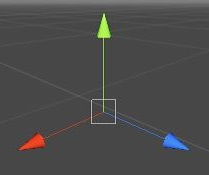
\includegraphics{img/transform.jpg}
\end{figure}
\section{World Environment}
The terrain editor also allows you to place foliage around the environment, trees, plants, grass and shrubs for example can be placed in great numbers relatively quick and efficiently.[~\cite{Scenes}] However, the amount of resources required steadily increases as more objects are placed into the scene, I've had to monitor the amount of draw calls required to run the scene. For instance; an object with one material equals a single draw call but a game object with four materials equals four draw calls. The GPU on a device would receive a 'hit' for every draw call requested, less draw calls means better performance equaling more fps at runtime.
\section{Game Objects}
On the topic of game objects, scripts written in either C-Sharp or JavaScript can at runtime instantiate game objects. For instance, I've used such scripts to spawn the player's animals in specific areas with vegetation. To give the animations from each of these animals some realistic purpose, the animation state engine allows the developer specify which animations play at certain times, for instance if a vegetation object was detected using a collision trigger component, a state machine variable could be set, thus allowing the animation engine known when to play the correct animations. For this project, I've used the very same methods to allow the player's character notify the animation engine when input from the virtual joystick is detected. The player controller script can independently control the speed of a specific animation, depending on the level of movement requested by the player.[~\cite{Game-Objects}] Input is taken from 'Virtual Axes', by default the Unity editor maps these axes in the 'Horizontal' and 'Vertical' planes to w, a, s, d and the arrow keys, this is usually more suitable to conventional games like FPS shooters. I've modified the virtual input controls in the input manager to suit the joystick library used to control the character in-game. By default, it's configured to suit a keyboard and mouse input.
\section{Lighting}
Another important aspect of game development is lighting, theres a number of options available within the Unity editor when developers want to simulate a specific mood or lighting effect to give the player more of a realistic setting to the environment. Scene textures can look completely different when lighting components like flares, spot lights and bounce reflections are applied correctly.[~\cite{Lighting}] For instance the following images taken from the Unity's docs web page shows how influential light can be to the environment.
\begin{figure}[!ht]
	\caption{Mood Lighting 1}
	\centering
	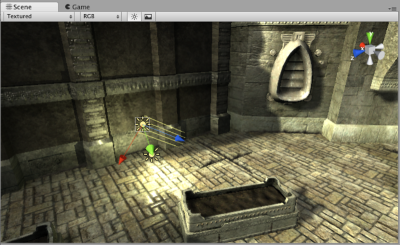
\includegraphics{img/light-mood-1.png}
\end{figure}
You can see how bright areas lit from the lighting components are, and how dark shadows are in contrast. Lighting is all about setting the correct mood for players to experience. Take the next figure, it's comprised of the exactly same scene with only the intensity and color of the lighting component being modified.
\begin{figure}[!ht]
	\caption{Mood Lighting 2}
	\centering
	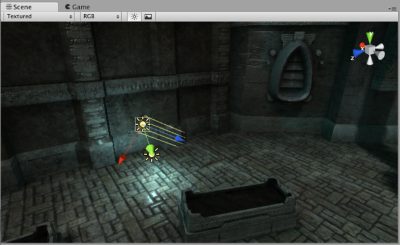
\includegraphics{img/light-mood-2.png}
\end{figure}
Lighting as you can see plays a major role in game development, for my own project I've applied only basic lighting techniques to the area of play because performance issues would incur and reduce the frame rate. Shadows have also been reduced quite considerably because of performance issues. As I stated before mobile devices rarely have enough resources to run with full shadows and lighting effects like flares, HDR or highly detailed shading.
\section{Rendering Detail}
The level of detail rendered on screen can be adjusted to suit the platform your targeting. The LOD or 'Level of Detail' from objects can vary depending on the main camera adjustment, for example if you set the view distance fairly low the render detail of objects in the game scene will change depending on how far the main camera is positioned away from a specific game object. A number of detail levels exist, ranging from 'LOD 0' which is stated to display the highest level of detail, while 'LOD 1' and 'LOD 2' are stated to be the lowest level of rendering. Developers can balance between these levels to find an acceptable level for the specific platform there targeting, especially when porting to mobile platforms with limited resources.
\section{Physics}
Convincing 3D physics behaviour is essential when creating an open world game. Game objects must have certain components to correctly accelerate, collied and react against other world objects. With just a few parameter settings you can easily simulate virtual objects just like the real thing, depending on what your creating of course.[~\cite{Physics}] Objects can be further manipulated using scripts written in either C-Sharp or JavaScript. For example if you wanted an object to behave like if it were in a low gravity environment and bounce around like a rubber ball it's quite simple as attaching a physics behaviour script to the object.
\section{Scripting}
Unity's scripting system is quite powerful, each game object usually has many different components with various responsibilities, for example rigidbodies, box colliders and hinge joints are used for physics simulation.[~\cite{Scripting}] These components can be influenced by scripts attached to the game object, for example if I wanted to move the game object all I would need to do is access the transform component using the following snippet.
\begin{minted}{csharp}
public class UsingOtherComponents : MonoBehaviour
{
  public GameObject otherGameObject;

  private AnotherScript anotherScript;
  private YetAnotherScript yetAnotherScript;
  private BoxCollider boxCol;

  void Awake ()
  {
    anotherScript = GetComponent<AnotherScript>();
    yetAnotherScript = otherGameObject.GetComponent<YetAnotherScript>();
    boxCol = otherGameObject.GetComponent<BoxCollider>();
  }
}
\end{minted}
Unity supports two different languages natively, C-Sharp and a JavaScript like language they call UnityScript. The .NET framework provides a powerful, stable and dependable foundation to your project's script writing. I believe is far easier to use an object orientated language for game development projects like the one I'm undertaking, as sections of the project can be split among teams of programmers. 
UnityScript is the other choice when implementing your game control logic, I would argue against using this language because in the long term adding new features and maintaining the source would become quite difficult as the complexity and size of the overall project expands.
\subsection{Script Behaviors}
One important aspect to be aware about when developing in the Unity SDK is that when each script created, by default inherits the 'MonoBehaviour' class. This class contains special methods that get called at specific times and events at runtime. For example, when the game becomes minimized to the background, a method named 'OnDisable' gets called before the application gets pushed to the background. I've used this method call to save the current state of the game to make sure player data is preserved if for instance the Android operating system closes the application. Similar methods exist like the 'OnEnable' is called within scripts when the application resumes for a suspended state, which is useful when restoring data that gets lost when the game gets suspended to the background.[~\cite{Script-Behaviours}]
The 'Awake' script behavior is used to initialize variables or any game state controls before the game starts and is only called once throughout it's lifetime instance. When all other objects have been initialized, the 'Awake' method is called so objects can safely communicate with one another. For example, its only possible to find other objects or query them when fully initialized. Each game object script using the 'Awake' method are all called randomly. Unity's developers recommend to use this functionality to setup references between scripts, and then use the 'Start' behavior to pass information from the script to subsequent scripts. 'Awake' method behaviors are always called before any 'Start' methods behaviors. Similar to the 'Awake' method, the 'Start' function is called once throughout the script's lifetime instance. It may not be called on the same frame as the 'Awake' behavior. When objects are instantiated at runtime, their 'Awake' method gets called after their 'Start' function. An example script with both the 'Start' and 'Awake' method implementations.
\begin{minted}{csharp}
public class ExampleClass : MonoBehaviour {
  private GameObject target;
  
  void Start() {
    target = GameObject.FindWithTag("Player");
  }
  
  void Awake() {
    Debug.Log("Target name: " + target.name);
  }
}
\end{minted}
There are many other types of behaviors that get fired at certain times, such as 'OnGUI', 'Update', 'FixedUpdate' and 'OnDestroy', plus many more are listed on the Unity docs reference.
\subsection{.NET Framework}
The Unity game engine utilizes the C-Sharp programming language. Backed by the latest .NET 4.6 framework, developers can take full advantage of the powerful and stable underlining libraries. 
The following sample is from the game controller class, which allows the player data to be saved using serialization. The library support is quite extensive, yet another reason why I've chosen to use Unity engine over other game engines like the Unreal 4 SDK.
Saving the Player's Data to File
\begin{minted}{csharp}
try
{
  FileStream file;
  BinaryFormatter bf = new BinaryFormatter();
  // Save player data
  file = File.Open(Application.persistentDataPath + 
    "/player.dat", FileMode.OpenOrCreate);
  bf.Serialize(file, _instance.player);
  file.Close();

  // Save cow data
  file = File.Open(Application.persistentDataPath + 
    "/cows.dat", FileMode.OpenOrCreate);
  bf.Serialize(file, _instance.cows);
  file.Close();
  Debug.Log ("Saving!");
}catch (UnityException e){
   Debug.Log("Saving Failed! - " + e);
}
\end{minted}
\section{Audio}
The audio system in Unity gives the developer complete control over how sounds are emitted by objects and heard by listeners. A game object with a sound component can attach a sound file to itself and play it with a degree of intensity and volume level. These sounds are picked up by 'Listener' components, which are usually attached to player controlled game objects. Sound can be emitted from audio sources either in a 2D or 3D form. Sound emitted in the 2D form is not usually used in 3D games as the sound has no fade control like 3D emitted sound contains. The fade distance is quite useful in simulating realistic ambient sounds effects.[~\cite{Audio-System}]
I’ve sourced a few sound effects from various places, all royalty free of course. To name a few sources, 'SoundCloud', 'FreeSound' and other various content providers on the Unity assets store.
\section{User Interface}
The user interface is an important feature of any game, it's critical to construct an efficient UI that gives the player a good impression of your game. UI elements in Unity are drawn upon a 'Canvas' component, and are drawn on screen in the same order as they appear in the hierarchy. If two elements overlap, the latest element drawn will sit on top of the other element. These 'Canvas' components have a special render mode setting, developers must choose one of these settings to display their GUI elements on screen. The render mode can either be set to screen space or world space. The 'Screen Space - Overlay' option places UI elements on top of the rendering scene, this allows UI components to resized automatically. While the 'Screen Space - Camera' option places the canvas a certain distance away from the main camera position. The UI elements are rendered by the camera component, which means it's settings affect the appearance of these elements and must be taken into account when developing the UI dimensions. If for instance the camera is set to 'Perspective', the UI elements that are rendered in this view, will be manipulated by the camera's field of view.[~\cite{UI-System}] If the camera or screen changes it's resolution, then the canvas will automatically resize itself and the elements drawn within it. The other rendering option available is the 'World Space' view, it displays UI elements with a 3D placement. It's a great tool for developers when they want to implement the user interface to make it feel part of the world view, rather then just being rendered on the user's screen. Usually these UIs are called a "diegetic interface". 
\chapter{System Design}
In this section of the document I'll cover the overall design and implementation of the game with help from UML diagrams to visualize the structure. Throughout this project I've had an object orientated design in mind, but in some cases I've done away with normal design principles for certain areas of the project. Unity's component structure requires the developer to implement the script's logic differently, compared to the normal OO compose and delegate structure of traditional design patterns. Unity's developers encourage use of the 'GetComponent' method of acquiring new instances of objects and scripts. Because of this variables inside of scripts usually will contain many 'public' access type variables and objects instances.
\subsection{Game Controller Design}
The game controller class provides quite an important function in the software design structure. It handles most of the main game control variables and object instances that are used throughout the software class structure. Another important class called 'CheckGC' basically checks at run if an instance of the game controller is present and valid, if no instance is found for some reason then one is created. The game itself can simply not function without one instantiated.
\begin{figure}[!ht]
	\caption{UML Diagram GC}
	\centering
	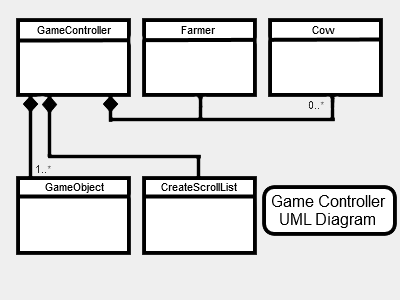
\includegraphics{img/gc_uml.png}
\end{figure}
As you can see below, I've included the different connections or relationships between these classes. The 'GameController' class fully composes each class found in the design image structure. Classes dependent on the variables inside of the 'GameController', access them through the use of a single static instance called 'instance' and will have it's variable 'set' parameter initialized to private. This will prevent outside classes from mishandling the variable and screwing up the game instance.
\subsection{Animal Controller Design}
Animals in the game require some form of behaviour and movement. The following UML diagram shows the basic aggregation relationship between the 'Cow' and 'CowController' classes. All of the animation and movement logic is contained within the 'CowController' class, also a simple state machine can be found in this class, because each cow object that's instantiated is essentially given its own thread and freedom in the game world. This state machine basically allows the individual animals in game to move and play specific animations when required.
\begin{figure}[!ht]
	\caption{UML Diagram CC}
	\centering
	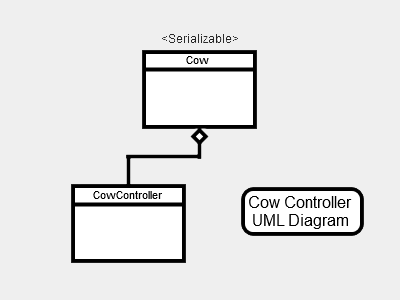
\includegraphics{img/cow_uml.png}
\end{figure}
The controller class also contains logic for a simple enough path finding algorithm that utilizes a Unity component called 'Raycasts' to detect objects around itself to avoid them and continue to a specific coordinate in the game world. I'm not sure if this really classifies as 'AI', but however the game animal object does attempt to seek the shortest path to the location specified. If the animal fails to find a route to the specific location it re-traces its steps to find another route.
This class also contains some control logic for the UI interface to display the correct information to the player when selected. This logic also controls the main camera view and translate it's position smoothly from one point to another without any glitching or laggy movement.
\subsection{Scene Control Design}
Each scene in the game has it's own controller script designed to keep track of items and elements instantiated in the game scene. Scripts controlling 3D scenes like the 'Farm' and 'Mart' scene, have external references to the static 'GameController' singleton instance and compose both the 'CameraController' and 'VCAnalogJoystickBase' classes. These classes allow the scene controller script access the main camera game object, to manipulate its movement and allows the virtual joystick to be displayed on screen, and also allow an external player controller script access input from virtual joystick class.
\begin{figure}[!ht]
	\caption{UML Diagram SC}
	\centering
	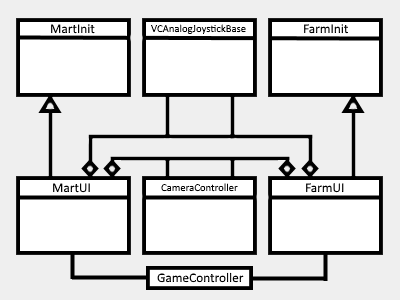
\includegraphics{img/scene_uml.png}
\end{figure}
When either the 'Farm' or 'Mart' scene starts to load, the initialization class first loads to setup the game scene. These classes set the initial spawn points the 'CowMaker' class uses to instantiate new animal objects in the game scene. If the spawner fails to create a new game object it will continue until a certain amount iterations. The 'FarmInit' class however has some extra functionality, it not only sets the spawn points for animal objects but also determines if the user requested to either load a previous saved game or create a new game entirely. 
Also during loading of the 'Mart' scene, static methods contained within 'BidderMaker' class are called to create a basic AI bidder the player competes against to buy cattle at the mart ring. Their positions are set to spawn around the ring, bidders will not bid on animals there not interested to buy, every bidder thats created at runtime is slightly different from one another. Its completely random, one bidder might be only interested in a specific breed , while another could be interested in all breeds. However, the weight of the animal can actually sway the AI to bid more money, a method contained within the 'Bidder' class called 'ConsiderBidding' determines how interested the agent is in the animal. I would say its a form of fuzzy logic that evaluates the current state of the game and then computes an AI interest level, if the value is quite high the AI put forward a good deal of money.
\subsection{Backend Design}
The application's backend relies on the 'Google Play Games' plugin that allows developers access an API that enables your game with some great features. These features include achievements, leaderboards, turn-based and real-time multiplayer. I've utilized both the leaderboard and achievement features in this project to improve the overall re-playability and engagement of the game. Developers can access the plugin on GitHub, and is completely open-source.[~\cite{GPG-Plugin}] The script class 'GPGController' contains the methods used to evaluate the player's achievements and progress in game. I've designed the controller's methods to be accessible statically from external classes, to keep the complexity to a minimum. There also another class called 'GoogleCon' that is auto generated when you initial setup the plugin, it contains static variables to the achievements, its not necessary to use these variables but they are useful. Another useful feature of this plugin is cloud saving and loading is available to the developer. Which could be convenient if the user games on multiple devices, this feature is only made available when the user logs into the service with their Google account. The plugin integrates Unity's social interface to display achievements and user progression on either the Android and iOS platform.
The following snippet of code is taken from the 'GPGController' class. It basically checks if the user has already logged in, but if the user is not, then it will ask if the user wishes to login by popping up a window, allowing the user to select a Google account to login into.
\begin{minted}{csharp}
public static void LoginIntoGPG()
{
  Debug.Log("Checking Login");
  Social.localUser.Authenticate((bool result) => {
    Debug.Log("Logged in?: " + result);
  });
}
\end{minted}
This method has a callback function that notifies the main execution thread when the user chooses to login or not, which can be handled by the 'result' variable. To check if the player has gotten an achievement or to post a high score, the method structurer is similar to the login method. First the value to be checked is passed into the method, then checks if the user is logged in and finally goes to the Google API to evaluate the variable.
\begin{minted}{csharp}
public static void CheckAchiev_1()
{
  Debug.Log("Checking CheckAchiev_1");
  Social.ReportProgress("CgkIuaLFq6kIEAIQBg", 100.0f, (bool result) => {
  Debug.Log("Achievement unlocked?: " + result);
});
}
\end{minted}
\chapter{System Evaluation}
Testing is an important task of any software project, without testing, programmers could introduce more bugs into the application when fixing or maintaining sections of the source code. It's important to test each section of application before signing off and releasing a new version of the program. Usually some form of automated testing is written to handle different classes and their subroutines to make sure nothing gets effected from the latest changes in the program. Unit testing is one such form that allows developers continually test as they work. The bundled IDE 'MonoDevelop' does support unit testing, so long as I keep C-Sharp as my main scripting language.
\subsection{Optimizing Graphics Performance}
Optimizing a game for the mobile platform is an important task for any game developer, especially when dealing with the problem of limited resources. Unity has a number of different tools available to diagnose bottlenecks and frame rate problems. The Unity 'Profiler Window' allows you see exactly whats using resources. It also displays how many draw calls are being requested for the GPU and how many CPU cycles required to run various areas of your game like collision detection, object physics and other CPU intensive calculations. I've used this tool to monitor the amount of resources over the project's development, interestingly enough Unity handles optimizations quite well. I've read that the render engine bundles similar textures into single draw calls reducing the load on a GPU. Even though I'm using relatively basic textures and models in my game, I still worry about frame rate problems, because every new object added to the game scene reduces the performance levels, I aim to target as many mobile devices as possible. The profiler displays data from the game in a timeline, and allows you to see which frames spike. The spikes signify an area of interest you need look into and inspect. The specific frames in these spikes areas in the graph need to be analyzed and debugged to see what component of the game is bottlenecking the application.
\subsection{Testing Hardware}
Mobile hardware ranges quite a lot when you start talking about all the different generations of iPhones and Android devices released to the consumer market over the last few years. While the Unity game engine allows you to target too many different platforms like PlayStation and Xbox, I’ve been mainly focusing my attention on the Android platform. This platform can present game development with a couple of problems, one would be the API level. Different versions of Android all the way from version 1.5 to latest of 6.0, presents one major problem to the developer. What API level do I develop for?, Unity thankfully handles this problem by allowing the developer to choose the lowest API level required to run the game.
Development hardware consisted of my own personal collection of Android devices, all with different screen sizes and API level versions. It’s quite simple to enable debugging on Android smartphones and tablet devices, the following method usually only applies to later models. Running an unsigned compiled APK file requires you to unlock the phone into developer mode, go into settings and navigate to the section 'About' and from there you should see an option for 'Software Information' or something similar, then 'More' if available and finally hit 'Build Number' seven times. Before I can build and compile the source into a APK file, I first must set or create the “keystore” file. It’s basically a signing certificate that must be included with the project when submitting applications to the Google play store. Also any incremental updates that proceed must also include this special file when building the project before submitting to the store.
\chapter{Conclusion}
Throughout this project I've learned quite a lot about game development, to only not brain storm ideas of gameplay but to implement them into a real project. I'll admit that the game is still in its early stages of development and does not provide any sort of solid storyline or dialog, it mainly gives you the general idea of what the game is about. During its development stage, I was still trying to grasp the tools and features available in Unity, if I were to restart the project tomorrow I would probably go about designing and implementing the game with a completely different method and approach.
During the implementation stage of the project I've learned a great deal about the Unity SDK. Everything from the lighting systems to audio components, making game development within Unity quite an enjoyable experience. With its simple drag and drop features, level creation and environment setup time is reduced considerably allowing developers to quickly prototype ideas and gameplay features.
Debugging in Unity was quite difficult to perform, especially when trying to figure out frame rate and performance issues. The included software IDE is a bit crude and flaky at times but it does perform tasks such as line breaking and remote debugging quite well without issue. The Android 'Logcat' tool has been extremely helpful throughout the project's development. It allows developers to remotely debug devices by observing the output logs from applications running.
I believe the game has plenty of potential to grow and develop into more than just another farm simulator game. From an education point of view the game could teach children about farm animals and how to properly care for them. Helpful tips and information could be displayed on screen occasionally to progressively teach the player about each animal as they play. 
Overall I've learned quite a lot from this project, both in visual and technical sides of Unity's SDK. Unity component structure at first was difficult to understand, it went against some design principles I've learned over the last few years. It took a considerable amount of time to properly grasp and implement an efficient software structure with Unity's unique component system, while keeping the game's performance at respectable levels.
\paragraph{Future Development}
\begin{itemize}
\item Gameplay features like private sales between the player and NPC's in-game could be an aspect to implement later in development, private sales between farmers take place occasionally. 
\item Multiplayer support may be included later in the project, which means likely that player chat, trading between players could be features implemented afterwards. 
\end{itemize}